\section{Ablation Studies}
\label{sec:abl}
We perform ablations across three main dimensions: architectures, modalities, and feature backbones.
When not mentioned, we adopt the defaults:
(i)~MViT trained on Kinetics400 dataset to represent video;
(ii)~ResNet50 trained on SFEW, FER, and VGGFace for character representations;
(iii)~fine-tuned RoBERTa for dialog utterance representations; and
(iv)~\modelname{} with appropriate masking to pick modalities or change the number of classifier tokens.

\begin{figure*}[t]
\centering
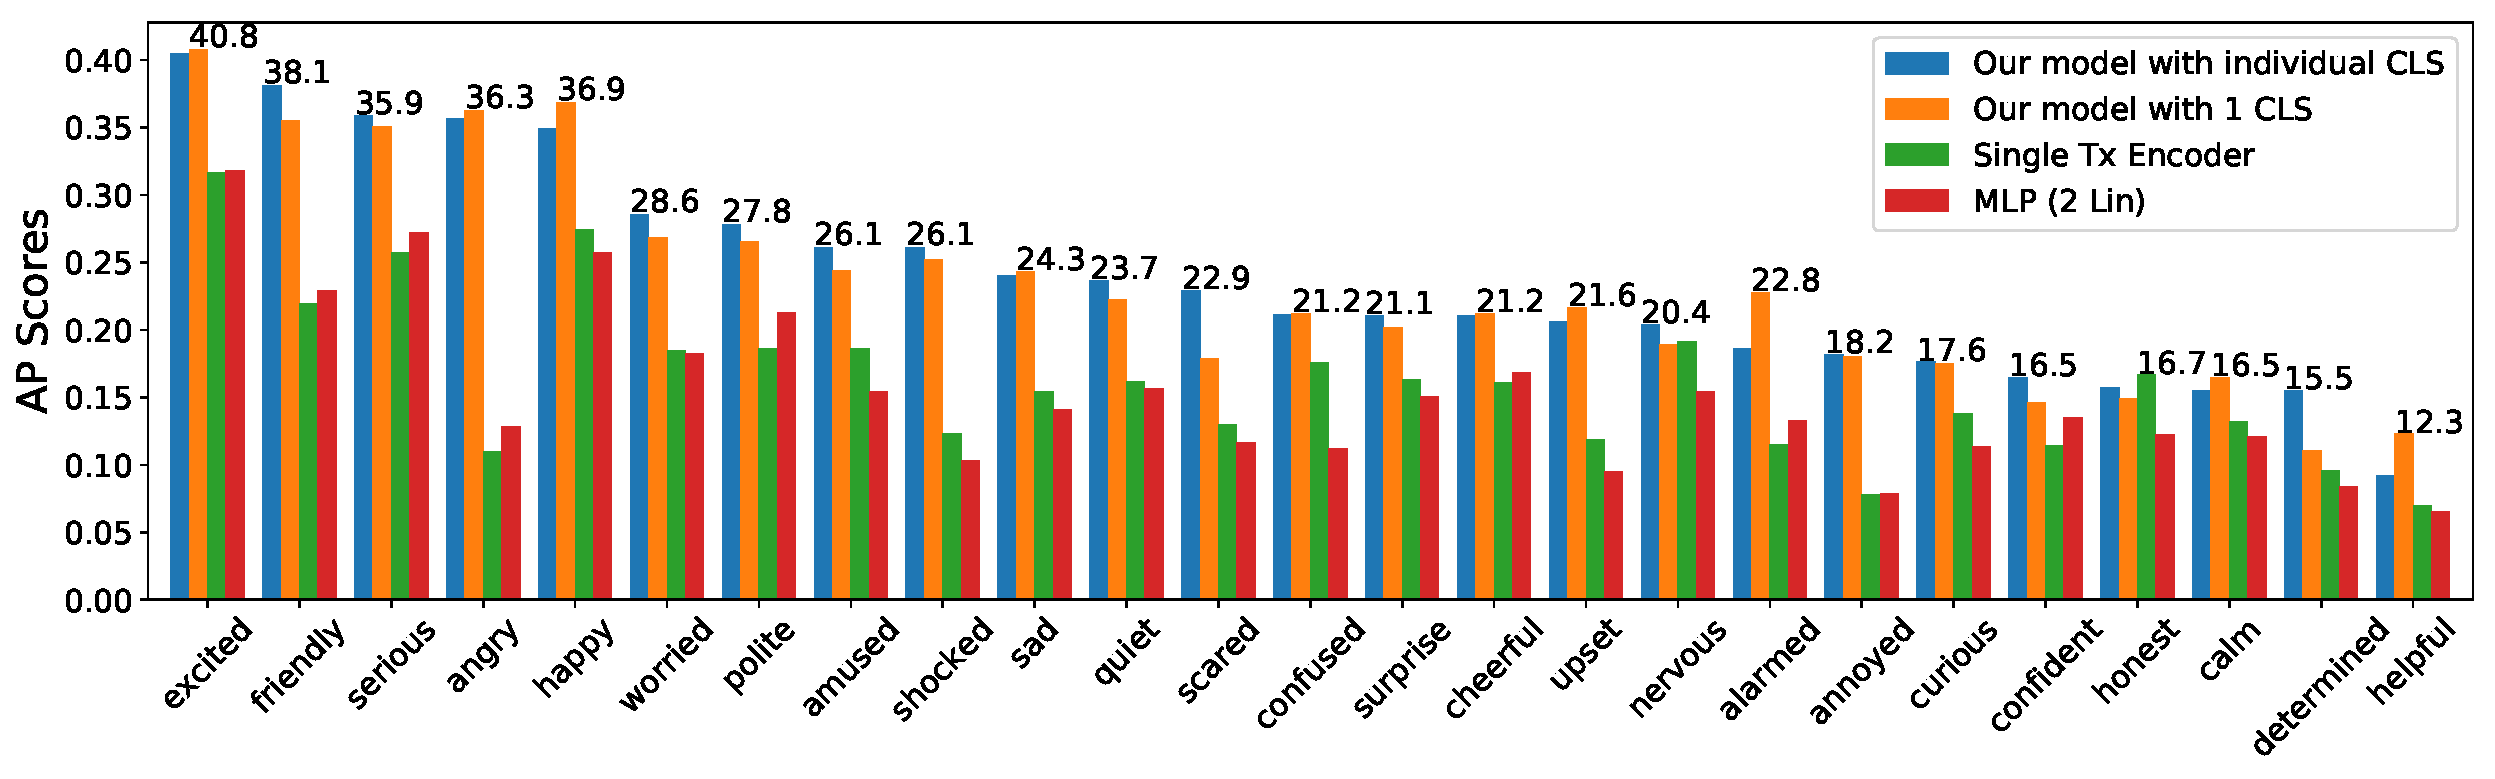
\includegraphics[width=1.05\linewidth,height=5cm]{Figures/t25_APs_sorted.pdf}
\vspace{-10mm}
\caption{Comparing scene-level per class AP of \modelname{} against baselines (Table~\ref{tab:arch_abl}) shows consistent improvements.
We also see that our model with $K$ classifier tokens outperforms the 1 CLS token on most classes.
AP of the best model is indicated above the bar.
Interestingly, the order in which emotions are presented is not the same as the frequency of occurrence (see~\ref{fig:emotionFrequency}).}
\vspace{-2mm}
\label{fig:per_class_ap}
\end{figure*}

\begin{table}[t]
\centering
\small
\tabcolsep=0.5cm
\begin{tabular}{l cc cc}
\toprule
\multicolumn{1}{c}{\multirow{2}{*}{Method}} & \multicolumn{2}{c}{Top-10} & \multicolumn{2}{c}{Top-25} \\
& Scene & Char  & Scene & Char  \\
\midrule
Random            & 16.87\scriptsize{$\pm$0.23} & 12.49\scriptsize{$\pm$0.15} & 9.73\scriptsize{$\pm$0.101} & 5.84\scriptsize{$\pm$0.05}  \\
\midrule
MLP (2 Lin)       & 23.94\scriptsize{{$\pm$}0.03} & 20.39\scriptsize{$\pm$0.01} & 15.26\scriptsize{{$\pm$}0.02} & 10.57\scriptsize{$\pm$0.02} \\
Single Tx encoder & 25.66\scriptsize{{$\pm$}0.02} & 20.95\scriptsize{$\pm$0.09} & 16.14\scriptsize{{$\pm$}0.03} & 11.08\scriptsize{$\pm$0.18} \\
\midrule
\modelname: 1 CLS & \emph{34.11}\scriptsize{$\pm$0.34} & \emph{23.81}\scriptsize{$\pm$0.24} & \emph{23.34}\scriptsize{$\pm$0.11} & 12.86\scriptsize{$\pm$0.11} \\
\modelname{} (Ours) & \textbf{34.22}\scriptsize{$\pm$0.18} & \textbf{24.35}\scriptsize{$\pm$0.23} & \textbf{23.86}\scriptsize{$\pm$0.10} & \textbf{13.36}\scriptsize{$\pm$0.11} \\
\bottomrule
\end{tabular}
\caption{Architecture ablation.
Emotions are predicted at both movie scene and individual character (Char) levels.
We see that our multimodal model significantly outperforms simpler baselines.
Best numbers in bold, close second in italics.}
\label{tab:arch_abl}
\end{table}

\begin{table}[t]
\centering
\small
\tabcolsep=0.3cm
\begin{tabular}{l cccc cccc}
\toprule
&\multirow{2}{*}{$V_r$} & \multirow{2}{*}{$V_m$} & \multirow{2}{*}{$D$} & \multirow{2}{*}{$C$} & \multicolumn{2}{c}{Top 10 (mAP)} & \multicolumn{2}{c}{Top 25 (mAP)} \\
&           &            &            &             & Scene           & Char           & Scene           & Char           \\
\midrule
1&\dingcheck &      -     &    -       &      -     & 22.81{\tiny $\pm$0.02} & 15.90{\tiny $\pm$0.19}& 14.85{\tiny $\pm$0.02} & 7.98{\tiny $\pm$0.05} \\
2&    -      & \dingcheck &    -       &      -     & 25.73{\tiny $\pm$0.02} & 17.88{\tiny $\pm$0.12}& 16.11{\tiny $\pm$0.05} & 8.96{\tiny $\pm$0.12} \\
3&    -      &      -     & \dingcheck &      -     & 27.28{\tiny $\pm$0.01} & 20.25{\tiny $\pm$0.14}& 20.20{\tiny $\pm$0.08} & 11.09{\tiny $\pm$0.12}\\
4&    -      &      -     &    -       & \dingcheck & 31.38{\tiny $\pm$0.40} & 21.22{\tiny $\pm$0.50}& 20.32{\tiny $\pm$0.05} & 11.23{\tiny $\pm$0.14}\\
\midrule
5&\dingcheck &      -     & \dingcheck &      -     & 27.19{\tiny $\pm$0.07} & 19.45{\tiny $\pm$0.10}& 19.72{\tiny $\pm$0.03} & 10.67{\tiny $\pm$0.08}\\
6&    -      & \dingcheck & \dingcheck &      -     & 28.93{\tiny $\pm$0.02} & 21.41{\tiny $\pm$0.15}& 21.29{\tiny $\pm$0.05} & 12.03{\tiny $\pm$0.23}\\  
7&    -      &      -     & \dingcheck & \dingcheck & 33.59{\tiny $\pm$0.10} & 23.54{\tiny $\pm$0.16}& 23.40{\tiny $\pm$0.09} & 13.01{\tiny $\pm$0.08}\\  
\midrule
8&\dingcheck &      -     & \dingcheck & \dingcheck & 33.60{\tiny $\pm$0.02} & 22.89{\tiny $\pm$0.02}& 22.76{\tiny $\pm$0.02} & 12.21{\tiny $\pm$0.02}\\
9&    -      & \dingcheck & \dingcheck & \dingcheck & \textbf{34.22} {\tiny $\pm$0.18} & \textbf{24.35}{\tiny $\pm$0.23}& \textbf{23.86}{\tiny $\pm$0.10} & \textbf{13.36}{\tiny $\pm$0.11}\\  
\bottomrule
\end{tabular}
\caption{
Modality ablation.
$V_{r}$: ResNet50 (Places365),
$V_{m}$: MViT (Kinetics400),
$D$: Dialog, and
$C$: Character.}
\label{tab:modal_abl}
\end{table}

\begin{table*}[tbp]
\centering
\tabcolsep=0.10cm
\begin{tabular}{l ccc | ccc | cc | cc cc}
\toprule
& \multicolumn{3}{c|}{Video} & \multicolumn{3}{c|}{Character} & \multicolumn{2}{c|}{Dialog} & \multicolumn{4}{c}{Metrics (mAP)} \\
& \multicolumn{1}{c}{MViT} & \multicolumn{1}{c}{R50} & \multicolumn{1}{c|}{R152} & \multicolumn{1}{c}{R50} & \multicolumn{1}{c}{VGG-M} & \multicolumn{1}{c|}{IRv1} & \multicolumn{1}{c}{RB} & \multicolumn{1}{c|}{RB} & \multicolumn{2}{c}{Top-10} & \multicolumn{2}{c}{Top-25} \\
& \multicolumn{1}{c}{K400} & \multicolumn{1}{c}{P365} & \multicolumn{1}{c|}{INet} & \multicolumn{1}{c}{FER} & \multicolumn{1}{c}{FER} & \multicolumn{1}{c|}{VGG-F} & \multicolumn{1}{c}{FT} & \multicolumn{1}{c|}{PT} & \multicolumn{1}{c}{Scene} & \multicolumn{1}{c}{Char} & \multicolumn{1}{c}{Scene} & \multicolumn{1}{c}{Char} \\ \midrule
1 & - & \dingcheck & - & - & - & \dingcheck & - & \dingcheck & 25.07\scriptsize{{$\pm$}0.12} & 15.48\scriptsize{{$\pm$}0.15} & 16.41\scriptsize{{$\pm$}0.24} & 8.31\scriptsize{{$\pm$}0.17} \\
2 & - & - & \dingcheck & - & - & \dingcheck & - & \dingcheck & 25.85\scriptsize{{$\pm$}0.24} & 15.63\scriptsize{{$\pm$}0.21} & 16.45\scriptsize{{$\pm$}0.09} & 8.31\scriptsize{{$\pm$}0.09} \\
3 & - & - & \dingcheck & - & \dingcheck & - & - & \dingcheck & 29.20\scriptsize{{$\pm$}0.22} & 19.88\scriptsize{{$\pm$}0.27} & 18.93\scriptsize{{$\pm$}0.38} & 10.16\scriptsize{{$\pm$}0.17} \\
4 & \dingcheck & - & - & - & - & \dingcheck & - & \dingcheck & 29.27\scriptsize{{$\pm$}0.08} & 18.07\scriptsize{{$\pm$}0.22} & 18.35\scriptsize{{$\pm$}0.09} & 0.09\scriptsize{{$\pm$}0.08} \\
5 & - & \dingcheck & - & - & \dingcheck & - & - & \dingcheck & 29.30\scriptsize{{$\pm$}0.21} & 19.73\scriptsize{{$\pm$}0.17} & 19.05\scriptsize{{$\pm$}0.19} & 10.31\scriptsize{{$\pm$}0.00} \\
6 & \dingcheck & - & - & - & \dingcheck & - & - & \dingcheck & 29.34\scriptsize{{$\pm$}0.08} & 20.50\scriptsize{{$\pm$}0.04} & 19.07\scriptsize{{$\pm$}0.19} & 10.34\scriptsize{{$\pm$}0.17} \\
7 & - & \dingcheck & - & - & - & \dingcheck & \dingcheck & - & 29.34\scriptsize{{$\pm$}0.17} & 19.49\scriptsize{{$\pm$}0.03} & 20.73\scriptsize{{$\pm$}0.08} & 10.75\scriptsize{{$\pm$}0.02} \\
8 & - & - & \dingcheck & - & - & \dingcheck & \dingcheck & - & 29.47\scriptsize{{$\pm$}0.14} & 19.29\scriptsize{{$\pm$}0.10} & 20.74\scriptsize{{$\pm$}0.11} & 10.79\scriptsize{{$\pm$}0.07} \\
9 & - & \dingcheck & - & \dingcheck & - & - & - & \dingcheck & 29.69\scriptsize{{$\pm$}0.38} & 20.25\scriptsize{{$\pm$}0.14} & 20.16\scriptsize{{$\pm$}0.29} & 11.06\scriptsize{{$\pm$}0.12} \\
10 & - & - & \dingcheck & \dingcheck & - & - & - & \dingcheck & 30.19\scriptsize{{$\pm$}0.38} & 20.27\scriptsize{{$\pm$}0.26} & 19.83\scriptsize{{$\pm$}0.07} & 11.06\scriptsize{{$\pm$}0.16} \\
11 & \dingcheck & - & - & \dingcheck & - & - & - & \dingcheck & 31.39\scriptsize{{$\pm$}0.34} & 21.18\scriptsize{{$\pm$}0.18} & 20.88\scriptsize{{$\pm$}0.28} & 11.46\scriptsize{{$\pm$}0.08} \\
12 & \dingcheck & - & - & - & \dingcheck & - & \dingcheck & - & 31.50\scriptsize{{$\pm$}0.36} & 21.60\scriptsize{{$\pm$}0.09} & 21.49\scriptsize{{$\pm$}0.30} & 11.64\scriptsize{{$\pm$}0.20} \\
13 & - & - & \dingcheck & - & \dingcheck & - & \dingcheck & - & 31.96\scriptsize{{$\pm$}0.20} & 21.81\scriptsize{{$\pm$}0.37} & 21.28\scriptsize{{$\pm$}0.25} & 11.58\scriptsize{{$\pm$}0.26} \\
14 & \dingcheck & - & - & - & - & \dingcheck & \dingcheck & - & 32.23\scriptsize{{$\pm$}0.07} & 21.45\scriptsize{{$\pm$}0.07} & 22.10\scriptsize{{$\pm$}0.11} & 11.63\scriptsize{{$\pm$}0.06} \\
15 & - & \dingcheck & - & - & \dingcheck & - & \dingcheck & - & 32.42\scriptsize{{$\pm$}0.26} & 22.32\scriptsize{{$\pm$}0.27} & 21.45\scriptsize{{$\pm$}0.17} & 11.62\scriptsize{{$\pm$}0.05} \\
16 & - & - & \dingcheck & \dingcheck & - & - & \dingcheck & - & 33.44\scriptsize{{$\pm$}0.33} & 22.89\scriptsize{{$\pm$}0.24} & 22.75\scriptsize{{$\pm$}0.18} & 12.52\scriptsize{{$\pm$}0.12} \\
17 & - & \dingcheck & - & \dingcheck & - & - & \dingcheck & - & 33.46\scriptsize{{$\pm$}0.21} & 22.98\scriptsize{{$\pm$}0.16} & 22.69\scriptsize{{$\pm$}0.22} & 12.48\scriptsize{{$\pm$}0.20} \\
18 & \dingcheck & - & - & \dingcheck & - & - & \dingcheck & - & \textbf{34.22}\scriptsize{{$\pm$}0.18} & \textbf{24.35}\scriptsize{{$\pm$}0.23} & \textbf{23.86}\scriptsize{{$\pm$}0.10} & \textbf{13.36}\scriptsize{{$\pm$}0.11} \\ \bottomrule
\end{tabular}
\caption{Extended feature ablations. The different feature backbones are 
(MViT, K400): MViT pretrained on Kinetics400,
(R50, P365): ResNet50 on Places365,
(R152, INet): ResNet152 on ImageNet,
(R50, FER): ResNet50 on Facial Expression Recognition (FER),
(VGG-M, FER): VGG-M on FER,
(IRv1, VGG-F): InceptionResNet-v1 trained on VGG-Face dataset,
(RB, FT): pretrained RoBERTa finetuned for emotion recognition and
(RB, PT): pretrained RoBERTa. Best numbers are in bold.}
\label{tab:feat_abl}
\end{table*}


\subsection{Architecture ablations}
\label{sec:abl:arch}
We compare our architecture against simpler variants in Table~\ref{tab:arch_abl}.
The first row sets the expectation by providing scores for a \emph{random} baseline
that samples label probabilities from a uniform random distribution between $[0, 1]$ with 100 trials.
Next, we evaluate \emph{MLP (2 Lin)}, a simple MLP with two linear layers with inputs as max pooled scene or character features.
An alternative to max pooling is self-attention.
The \emph{Single Tx encoder} performs self-attention over features (as tokens) and a classifier token to which a multi-label classifier is attached.
Both these approaches are significantly better than random, especially for individual character level predictions which are naturally more challenging than scene-level predictions. Finally, we compare multimodal \modelname{} that uses 1 classifier token to predict all labels (\modelname: 1 CLS) against $K$ classifier tokens (last row).
Both models achieve significant improvements, \eg~in absolute points, +8.5\% for Top-10 scene labels and +2.3\% for the much harder Top-25 character level labels.
We believe the improvements reflect \modelname{}'s ability to encode multiple modalities in a meaningful way.
Additionally, the variant with $K$ classifier tokens (last row) shows small but consistent +0.5\% improvements over 1 classifier token on Top-25 emotions.

Fig.~\ref{fig:per_class_ap} shows the scene-level AP scores for the Top-25 labels.
Our model outperforms the MLP and Single Tx encoder on 24 of 25 labels and outperforms the single classifier token variant on 15 of 25 labels.
\modelname{} is good at recognizing expressive emotions such as \emph{excited, serious, happy} and even mental states such as \emph{friendly, polite, worried}.
However, other mental states such as \emph{determined} or \emph{helpful} are challenging.


\subsection{Modality ablations}
\label{sec:abl:modality}
We evaluate the impact of each modality (video, characters, and utterances) on scene- and character-level emotion prediction in Table~\ref{tab:modal_abl}.
We observe that the character modality (row 4, R4) outperforms any of the video or dialog modalities (R1-R3).
Similarly, dialog features (R3) are better than video features (R1, R2), common in movie understanding tasks~\cite{moviegraphs, movieqa}.

Interistingly, we also observe that having additional modality does not always help and the choice of feature backbone is important to get the desired results.
Scene features $V_r$, extracted from ResNet50 pretrained on Places365 dataset, which are more representative of the environment where the movie scenes may be happening, are consistently worse than action features $V_m$, which are extracted from a MViT\_v1 model pretrained on Kinetics400 dataset and is expected to be more representative of the actions happening within the movie scenes. Comparing R1, R2 or R5, R6 or R8, R9 reflect that $V_m$ assists model and works well with character and scene modalities for emotion recognition whereas $V_r$ makes it difficult for model to desipher emotions.

Finally, our observations reveal that the utilization of all modalities (R9) yields superior performance compared to other combinations. This outcome strongly suggests that the task of emotion recognition is inherently multimodal.

\subsection{Backbone ablations}\
\label{sec:abl:backbones}
We compare several backbones for the task of emotion recognition. \\
(i) MViT\_V1 model~\cite{FanMViT2021} pre-trained on Kinetics400~\cite{CarreiraQuoVadis2017} dataset, ResNet50~\cite{resnet} pre-trained on Places365 dataset~\cite{places365} and ResNet152~\cite{resnet} pre-trained on ImageNet dataset~\cite{imagenet} for video features.\\
(ii) ResNet50~\cite{facefeat} pre-trained on FER~\cite{fer13}, SFEW~\cite{sfew} and VGGFace~\cite{vggface} datasets, VGG-m~\cite{facefeat} pre-trained on FER13~\cite{fer13} dataset and InceptionResNetV1~\cite{SzegedyInceptionNet2015} pre-trained on VGGFace2~\cite{CaoVGGF22018} dataset for character features; and \\
(iii) A pre-trained and finetuned version on RoBERTa for dialogue features.

The effectiveness of the fine-tuned RoBERTa model is evident by comparing pairs of rows R6, R12 and R5, R15 and R3, R13 of Table~\ref{tab:feat_abl}, where we see a consistent improvement of 1-3\%.
Character representations with ResNet50-FER show improvement over VGGm-FER as seen from R11, R18 or R15, R17.
Finally, comparing R17, R18 shows the benefits provided by action features as compared to places.

In conclusion, ResNet50 trained on FER appears to be a good representation for characters, and the MViT trained on Kinetics400 provides better results for both the label sets, while ResNet50 trained on Places365 is a close second.

\subsection{SoTA Comparison}
\label{sec:sota}

\begin{table*}[t]
\centering
\tabcolsep=0.07cm
\begin{tabular}{l cc cc cc}
\toprule
\multicolumn{1}{c}{\multirow{2}{*}{Method}} & \multicolumn{2}{c}{Top 10}      & \multicolumn{2}{c}{Top 25}      & \multicolumn{2}{c}{Emotic}      \\
\multicolumn{1}{c}{} & Val   & Test  & Val   & Test  & Val   & Test  \\ \midrule
Random               & 16.87\scriptsize{{$\pm$}0.23} & 13.84\scriptsize{{$\pm$}0.20} & 9.73\scriptsize{{$\pm$}0.10} & 7.57\scriptsize{{$\pm$}0.08} & 11.47\scriptsize{{$\pm$}0.11} & 11.36\scriptsize{{$\pm$}0.09} \\
CAER~\cite{caer}
& 18.35\scriptsize{{$\pm$}0.10} & 15.38\scriptsize{{$\pm$}0.13} & 11.84\scriptsize{{$\pm$}0.07} & 9.49\scriptsize{{$\pm$}0.08}  & 13.91\scriptsize{{$\pm$}0.06} & 12.68\scriptsize{{$\pm$}0.02} \\
ENet~\cite{WeiEmotionNet}
& 19.14\scriptsize{{$\pm$}0.10} & 16.14\scriptsize{{$\pm$}0.05} & 11.22\scriptsize{{$\pm$}0.06} & 9.08\scriptsize{{$\pm$}0.08}  & 13.55\scriptsize{{$\pm$}0.06} & 12.64\scriptsize{{$\pm$}0.03} \\
AANet~\cite{attendaffectnet}
& 21.55\scriptsize{{$\pm$}0.18} & 17.55\scriptsize{{$\pm$}0.16} & 12.55\scriptsize{{$\pm$}0.15} & 10.20\scriptsize{{$\pm$}0.13} & 14.71\scriptsize{{$\pm$}0.19} & 13.37\scriptsize{{$\pm$}0.20} \\
M2Fnet~\cite{m2fnet}
& 24.55\scriptsize{{$\pm$}0.39} & 19.10\scriptsize{{$\pm$}0.06} & 16.02\scriptsize{{$\pm$}0.14} & 13.05\scriptsize{{$\pm$}0.31} & 18.27\scriptsize{{$\pm$}0.16} & 16.76\scriptsize{{$\pm$}0.20} \\
\midrule
\modelname{}  & \textbf{34.22}\scriptsize{{$\pm$}0.18} & \textbf{29.35}\scriptsize{{$\pm$}0.18} & \textbf{23.86}\scriptsize{{$\pm$}0.10} & \textbf{19.47}\scriptsize{{$\pm$}0.10} & \textbf{23.67}\scriptsize{{$\pm$}0.03} & \textbf{21.40}\scriptsize{{$\pm$}0.03} \\ \bottomrule
\end{tabular}
\vspace{-3mm}
\caption{Comparison against SoTA for scene-level predictions. \emph{AANet} denotes AttendAffectNet, while \emph{ENet} refers to EmotionNet.}
\label{tab:sota_scene_abl}
\end{table*}

\begin{table*}[t]
\centering
\tabcolsep=0.09cm
\begin{tabular}{l cc cc cc}
\toprule
\multicolumn{1}{c}{\multirow{2}{*}{Method}} & \multicolumn{2}{c}{Top 10}      & \multicolumn{2}{c}{Top 25}      & \multicolumn{2}{c}{Emotic}      \\
\multicolumn{1}{c}{} & Val   & Test  & Val   & Test & Val   & Test \\
\midrule
Random
& 12.49\scriptsize{{$\pm$}0.15} & 11.37\scriptsize{{$\pm$}0.14} & 5.84\scriptsize{{$\pm$}0.05} & 5.36\scriptsize{{$\pm$}0.05} & 6.40\scriptsize{{$\pm$}0.05} & 6.32\scriptsize{{$\pm$}0.05} \\
AANet~\cite{attendaffectnet}
& 17.43\scriptsize{{$\pm$}0.28} & 16.04\scriptsize{{$\pm$}0.19} & 8.64\scriptsize{{$\pm$}0.19} & 7.20\scriptsize{{$\pm$}0.15} & 8.53\scriptsize{{$\pm$}0.17} & 7.75\scriptsize{{$\pm$}0.11} \\
M2Fnet~\cite{m2fnet}
& 20.82\scriptsize{{$\pm$}0.28} & 19.01\scriptsize{{$\pm$}0.45} & 10.67\scriptsize{{$\pm$}0.38}  & 9.71\scriptsize{{$\pm$}0.34} & 11.30\scriptsize{{$\pm$}0.35}  & 9.92\scriptsize{{$\pm$}0.02} \\
\midrule
\modelname{} (Ours)
& \textbf{24.35}\scriptsize{{$\pm$}0.23} & \textbf{22.31}\scriptsize{{$\pm$}0.11} & \textbf{13.36}\scriptsize{{$\pm$}0.11} & \textbf{11.71}\scriptsize{{$\pm$}0.05} & \textbf{12.29}\scriptsize{{$\pm$}0.08} & \textbf{11.76}\scriptsize{{$\pm$}0.10} \\ \bottomrule
\end{tabular}
\vspace{-2mm}
\caption{Comparison against SoTA for character-level predictions. \emph{AANet} denotes AttendAffectNet.}
\label{tab:char_sota_abl}
\end{table*}


We compare our model against published works 
EmotionNet~\cite{WeiEmotionNet},
CAER~\cite{caer}, 
AttendAffectNet~\cite{attendaffectnet}, and
M2Fnet~\cite{m2fnet}
by adapting them for our tasks.

\paragraph{EmotionNet}~\cite{WeiEmotionNet}
employs a joint embedding training approach that aligns learned text embeddings, obtained through the word2vec model~\cite{MikolovWord2Vec}, with image embeddings extracted from a ResNet50 backbone. For our adaptation, we utilize the same backbones. Since we use video as input, the frame features are max-pooled to generate a consolidated representation. The embedding loss is applied, with emotion labels serving as keywords for joint embedding training. The ResNet50 is then fine-tuned for multilabel emotion recognition, where individual frame features undergo max-pooling before reaching the logits layer.

\paragraph{CAER (Context Aware Emotion Recognition)}~\cite{caer}
is a deep Convolutional Network which consists of two stream encoding networks to separately extract the facial and context features which are fused using an adaptive fusion network.
Detections from our extended face tracks are used as inputs for the face encoding stream and the full video frame with masked faces was used as input to context encoding stream.
Since CAER is designed to extract emotions from images we adapt it to videos by applying max-pooling over the fused features from both the streams to generate a single representation for a video.
This adapted model is trained to predict multiple scene-level emotions.

\paragraph{M2FNet}~\cite{m2fnet}
is a transformer based model originally developed for Emotion Recognition in Conversations (ERC) and features a fusion-attention mechanism to modulate the attention given to each utterance considering the audio and visual features.
As this model is designed for utterance emotion recognition we apply a max-pooling operation over the final outputs of fusion attention module to generate a feature representation for all the utterances in a video.
Since this model provides two strategies to consider visual features: one with the video frame and another that combines multiple faces in a frame, we use them to predict either scene- or character-level emotions separately.

\paragraph{AttendAffectNet}~\cite{attendaffectnet}
proposes two multi-modal self-attention based approaches for predicting emotions from movie clips. We adapted the proposed Feature AttendAffectNet model in our work.
It leverages the transformer encoder block where every input token represents a different modality. These modality feature vectors are generated by average pooling over respective features. Following the proposed mechanism, a classification head was attached at the end of the model for predicting multi-label emotions.
We adopt the same backbone representations, MViT~\cite{FanMViT2021} pre-trained on Kinetics400~\cite{CarreiraQuoVadis2017} and ResNet50 pretrained on FER13~\cite{fer13}, for their work to extract scene and face features respectively.

Table~\ref{tab:sota_scene_abl} shows scene-level performance while the character-level performance is presented in Table~\ref{tab:char_sota_abl}.
First, we note that the test set seems to be harder than val as also indicated by the random baseline, leading to a performance drop from val to test across all approaches.
\modelname{} outperforms all previous baselines by a healthy margin.
For scene level, we see +4.6\% improvement on Emotic labels, +7.8\% on Top-25, and +9.7\% on Top-10.
Character-level predictions are more challenging, but we see consistent improvements of +1.5-3\% across all label sets.
Matching expectation, we see that simpler models such as EmotionNet or CAER perform worse than Transformer-based approaches of M2Fnet and AttendAffectNet.
Note that EmotionNet and CAER are challenging to adapt for character-level predictions and are not presented, but we expect M2Fnet or AttendAffectNet to outperform them.
